% !TeX document-id = {0be8c18c-9430-4e9a-bdd9-12beadebfebc}
% !TeX TXS-program:bibliography = txs:///biber
\documentclass[11pt]{beamer}
\uselanguage{portuguese}
\languagepath{portuguese}
\deftranslation[to=portuguese]{Theorem}{Teorema}
\deftranslation[to=portuguese]{theorem}{teorema}
\deftranslation[to=portuguese]{Example}{Exemplo}
\deftranslation[to=portuguese]{example}{exemplo}
\deftranslation[to=portuguese]{Lemma}{Lema}
\deftranslation[to=portuguese]{lemma}{Lema}
\deftranslation[to=portuguese]{Corollary}{Corolário}
\deftranslation[to=portuguese]{corollary}{corolário}
%\deftranslation[to=portuguese]{and}{e}

\usepackage[brazilian]{babel}
\usepackage[utf8]{inputenc}
\usepackage[T1]{fontenc}
\usepackage{lmodern}
\usepackage{amsmath}
\usepackage{amssymb}
\usepackage{mathtools}
\usepackage{color}
\usepackage{pgfplots}
\usepackage{tikz}
\usepackage{subcaption}
%\usepackage{appendixnumberbeamer}

\newenvironment{transitionframe}{
	\setbeamercolor{background canvas}{bg=yellow}
	\begin{frame}}{
	\end{frame}
}
\usetheme{default}
\usefonttheme{structuresmallcapsserif}

%% I use a beige off white for my background
\definecolor{MyBackground}{RGB}{255,253,218}
\useinnertheme[shadow]{rounded}
\setbeamercolor{block title}{bg=MyBackground}
\setbeamercolor{block body}{bg=MyBackground}
\setbeamercolor{example title}{bg=MyBackground}
\setbeamercolor{example body}{bg=MyBackground}


\newcommand{\blue}[1]{\textcolor{blue}{#1}}
\newcommand{\red}[1]{\textcolor{red}{#1}}
\newcommand{\purple}[1]{\textcolor{purple}{#1}}
\newcommand{\gray}[1]{\textcolor{gray}{#1}}
\setbeamertemplate{navigation symbols}{}
%\setbeamertemplate{page number in head/foot}[appendixframenumber]

%\usepackage{graphics}
\usepackage{graphicx}

\definecolor{blue_emph}{RGB}{0,114,178}
\definecolor{red}{RGB}{213,94,0}
\definecolor{yellow}{RGB}{240,228,66}
\definecolor{green}{RGB}{0,158,115}
\definecolor{purple}{RGB}{204,121,167}
\definecolor{orange}{RGB}{230,159,0}
\definecolor{lightblue}{RGB}{86,180,233}

%\setbeamercolor{frametitle}{fg=blue}
%\setbeamercolor{title}{fg=blue}
\setbeamertemplate{footline}[frame number]
\setbeamertemplate{navigation symbols}{} 
\setbeamertemplate{itemize items}{-}
%\setbeamercolor{itemize item}{fg=blue}
%\setbeamercolor{itemize subitem}{fg=blue}
\setbeamertemplate{enumerate items}[default]
%\setbeamercolor{enumerate subitem}{fg=blue}
\setbeamercolor{button}{bg=MyBackground,fg=blue}
\usefonttheme{structuresmallcapsserif}

%\setbeamercolor{section in toc}{fg=blue}
%\setbeamercolor{subsection in toc}{fg=red}
\setbeamersize{text margin left=1em,text margin right=1em} 


\usepackage{appendixnumberbeamer}

\usepackage[
backend=biber,
style=authoryear,
natbib=true
]{biblatex}
\addbibresource{../bibliography.bib}

\newenvironment{wideitemize}{\itemize\addtolength{\itemsep}{10pt}}{\enditemize}
\newenvironment{wideenumerate}{\enumerate\addtolength{\itemsep}{10pt}}{\endenumerate}
\newenvironment{halfwideitemize}{\itemize\addtolength{\itemsep}{0.5em}}{\enditemize}
\newenvironment{halfwideenumerate}{\enumerate\addtolength{\itemsep}{0.5em}}{\endenumerate}


\author{Luis A. F. Alvarez}
\title{EAE1223: Econometria III}
\subtitle{Aula 3 - Decomposições descritivas de séries de tempo}
%\logo{}
%\institute{}
\date{\today}
%\subject{}
%\setbeamercovered{transparent}

\begin{document}

\begin{frame}[plain]
	\maketitle
\end{frame}

\begin{frame}{Decomposição aditiva de uma série de tempo}
	\begin{halfwideitemize}
		\item Podemos considerar o seguinte modelo para uma série de tempo $X_t$, $t \in \mathcal{T}$:
		\begin{equation}
			X_t = 	T_t + C_t + S_t + U_t
		\end{equation}
		onde
		\begin{halfwideenumerate}
			\item $T_t$ é a {\color{blue}tendência} de $X$. Movimento de longo prazo da série.
			\item $C_t$ é o {\color{blue}ciclo} de $X$. Movimento oscilatório em torno da tendência de frequência, em geral, desconhecida.
			\item $S_t$ é a {\color{blue}sazonalidade} de $X$. Movimento oscilatório de periodicidade bem-definida.
			\begin{halfwideitemize}
				\item Vendas no comércio costumam apresentar alta nos meses de maio e dezembro.
			\end{halfwideitemize}
			\item $U_t$ é o {\color{blue}componente idiossincrático} da série $X$ em $t$. Captura fenômenos específicos a $t$ e não explicados pelos demais componentes.
		\end{halfwideenumerate}
	\end{halfwideitemize}
\end{frame}

\begin{frame}{Decomposição multiplicativa de uma série}
	\begin{halfwideitemize}
		\item Podemos considerar o seguinte modelo para uma série de tempo $X_t$, $t \in \mathcal{T}$:
		\begin{equation}
			X_t = 	T_t \cdot C_t \cdot S_t \cdot U_t
		\end{equation}
		onde os componentes são definidos como no modelo aditivo.
		\item Um modelo multiplicativo implica um modelo aditivo em \text{log}.
		\begin{equation}
			\log(X_t) = \tau_t + c_t + s_t + u_t
		\end{equation}
		\vspace{-1em}
		\begin{itemize}
			\item Estimação é feita trabalhando com modelo aditivo em log.
		\end{itemize}
		\item Observe que, no modelo multiplicativo, a tendência afeta a {\color{blue}escala} das variáveis.
		\begin{halfwideitemize}
			\item Em particular, esperamos que, no modelo multiplicativo, a variância de $\Delta X_t = X_{t} - X_{t-1}$ mude bastante com o tempo.
			\item Escolha entre modelo aditivo ou multiplicativo pode ser feita observando um gráfico de $\Delta X_t = X_{t} - X_{t-1}$.
		\end{halfwideitemize}
	\end{halfwideitemize}
\end{frame}

\begin{frame}{Modelo aditivo (nível e primeira diferença)}
	\begin{figure}
		\begin{subfigure}{0.45\textwidth}
			\centering
			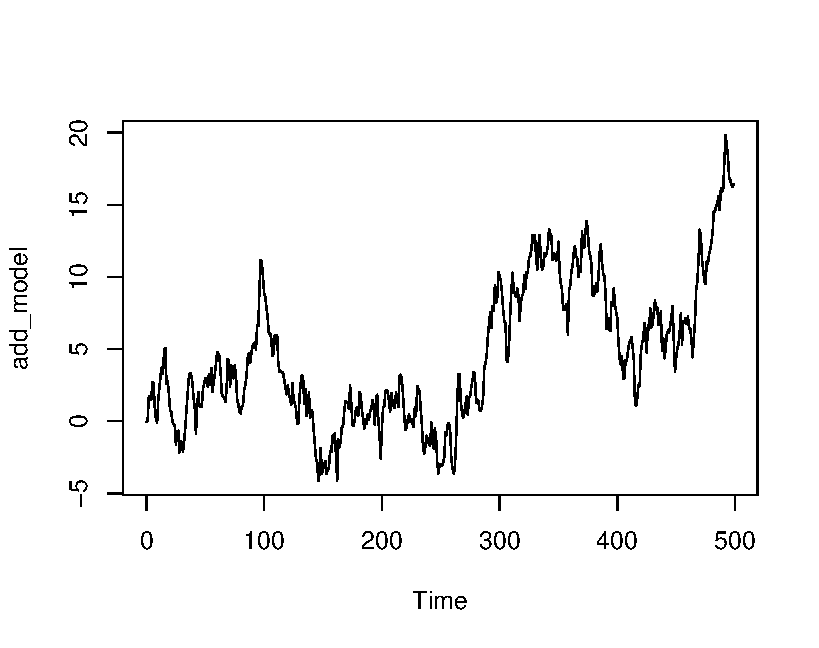
\includegraphics[scale=0.4]{graficos/aditivo_nivel.pdf}
			\caption{Nível}
\end{subfigure}
		\begin{subfigure}{0.45\textwidth}
	\centering
	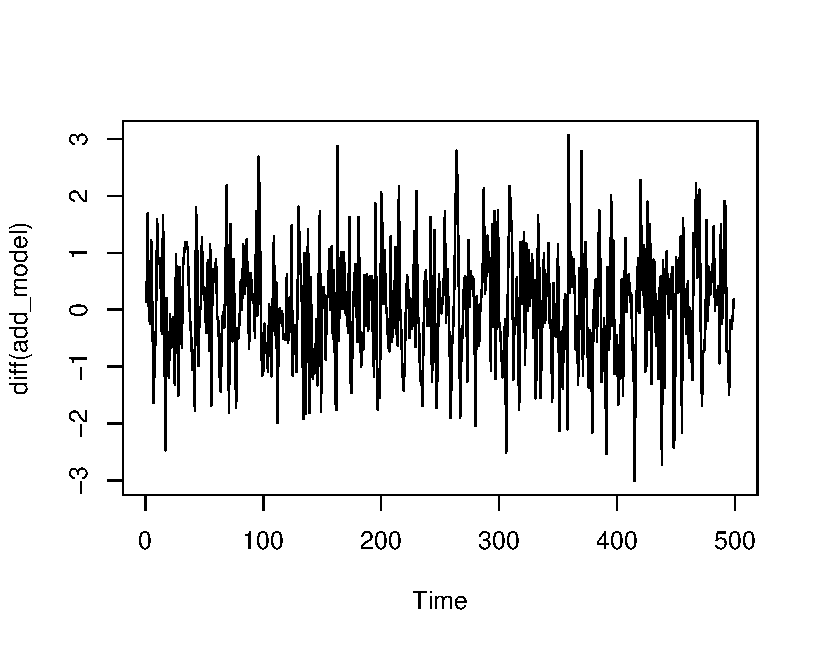
\includegraphics[scale=0.4]{graficos/aditivo_diff.pdf}
	\caption{Primeira diferença}
\end{subfigure}
	\end{figure}
\end{frame}


\begin{frame}{Modelo multiplicativo (nível e primeira diferença)}
	\begin{figure}
		\begin{subfigure}{0.45\textwidth}
			\centering
			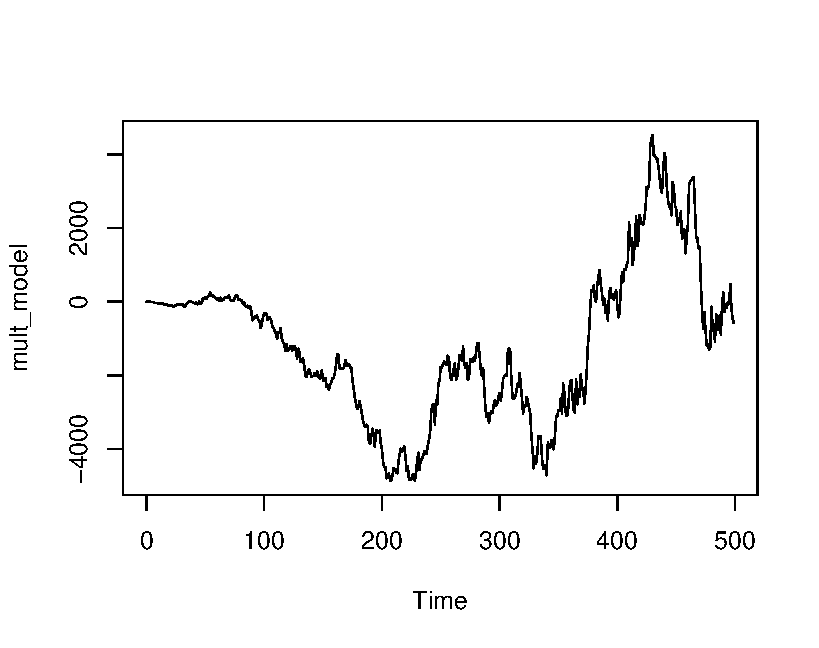
\includegraphics[scale=0.4]{graficos/multiplicativo_nivel.pdf}
			\caption{Nível}
		\end{subfigure}
		\begin{subfigure}{0.45\textwidth}
			\centering
			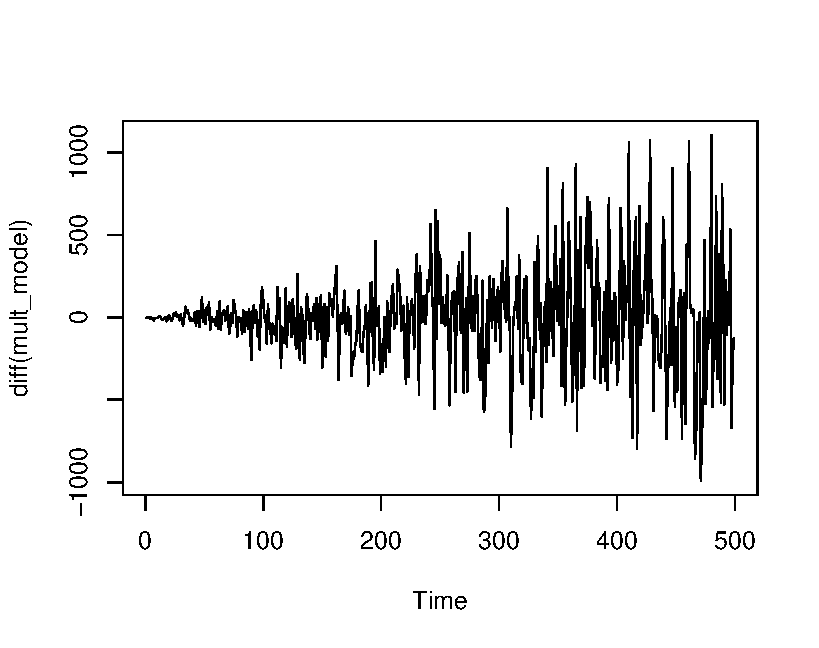
\includegraphics[scale=0.4]{graficos/multiplicativo_diff.pdf}
			\caption{Primeira diferença}
		\end{subfigure}
	\end{figure}
\end{frame}
\begin{frame}{Ajuste sazonal}
	\begin{halfwideitemize}
		\item Remoção do componente sazonal clássica faz uso de {\color{blue}médias móveis}.
		\item Suponha que a série tem movimentos sazonais bem definidos a cada $h$ períodos, onde $h$ é número \textbf{ímpar} (e.g. sazonalidade semanal numa série diária). Podemos construir a {\color{blue} média móvel centrada em $t$} como:
		\begin{equation}
			\tilde{X}_t = \frac{1}{h}\sum_{s = t - (h-1)/2}^{t+(h-1)/2} X_s
		\end{equation}
		\item O {\color{blue}fator de correção sazonal} para $s=1,\ldots, h$ é dado por:
		\begin{equation}
			\hat{\delta}_s = \frac{1}{\lfloor (T - s)/h\rfloor + 1}\sum_{t = s, s + h, s+ 2h \ldots} (X_t - \tilde{X}_t)
		\end{equation}
		\item E o fator recentrado é:
		\begin{equation}
			\tilde{\delta}_s = \hat{\delta}_s - \frac{1}{h}\sum_{j=1}^h \hat{\delta}_j		
		\end{equation}

		
	\end{halfwideitemize}
	
\end{frame}

\begin{frame}{Ajuste sazonal (cont.)}
	\begin{itemize}
				\item Fatores podem ser usado para obter séries corrigidas da sazonalidade, subtraindo-se de cada observação  o $\tilde{\delta}_s$ correspondente.
		\item Se $h$ é par, calculamos $\tilde{X}_t$ combinando duas médias não centradas:
		$$			\tilde{X}_t =0.5 \times \frac{1}{h}\sum_{s = t - (h-2)/2 {\color{red}- 1}}^{t+(h-2)/2} X_t + 0.5 \times \frac{1}{h}\sum_{s = t - (h-2)/2 - 1}^{t+(h-2)/2{\color{red}+1}} X_t $$
	\end{itemize}
\end{frame}

\begin{frame}{Exemplo: taxa de desemprego mensal no Brasil}
	\begin{figure}
		\caption{Taxa de desemprego original (preto) e com ajuste via médias móveis centradas (azul)}
		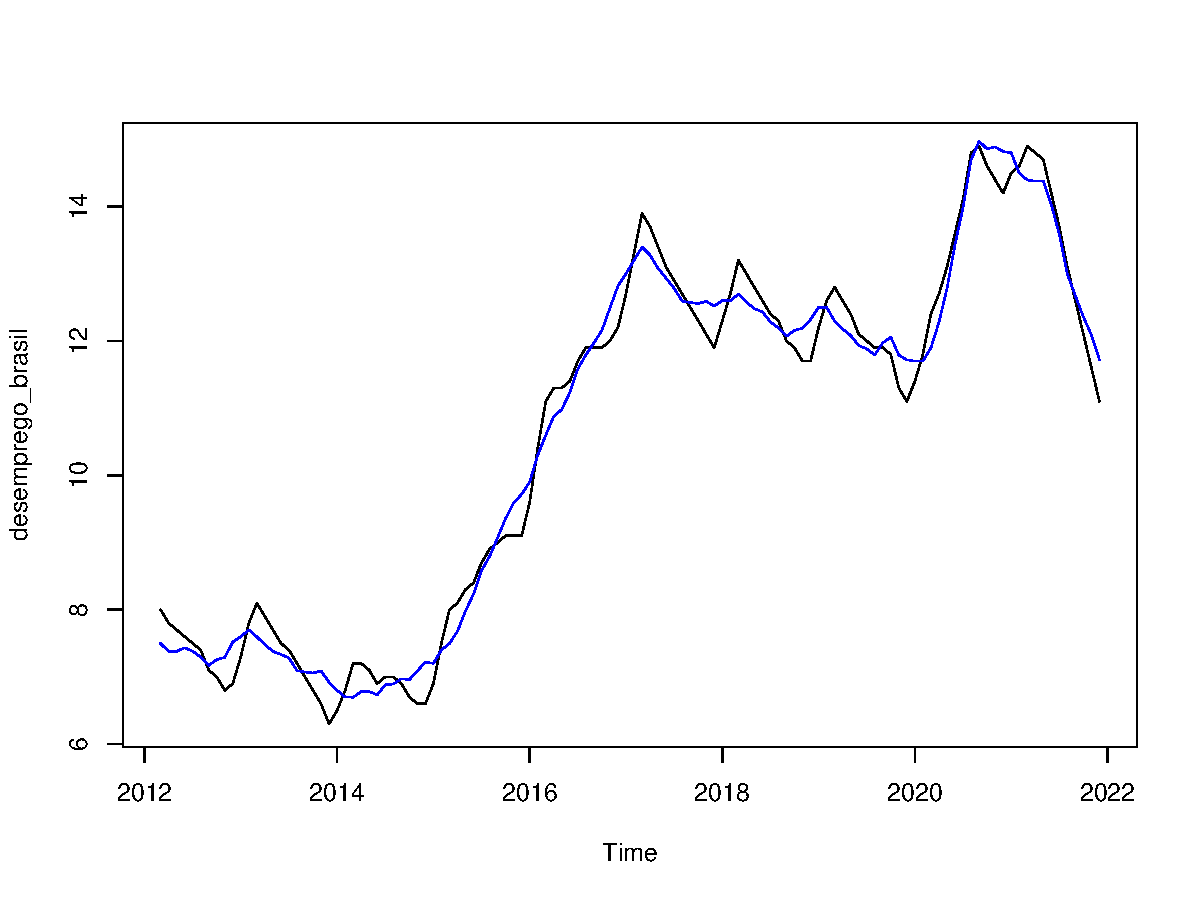
\includegraphics[scale=0.4]{graficos/desemprego_mm.pdf}
	\end{figure}
\end{frame}

\begin{frame}{X13 Arima-Seats}
	\begin{wideitemize}
		\item Metodologia de ajuste sazonal desenvolvida pelo \textit{US Census Bureau}.
		\item Padrão ouro para ajustes sazonais.
		\begin{halfwideitemize}
			\item Combina metodologia de médias móveis com a possibilidade de inclusão de efeitos-calendário (por padrão, modelo controla por dias úteis do mês e alguns feriados móveis; passível de alteração), detecção automática de \textit{outliers}, \textit{backfitting} para completamento da série de tempo e seleção automática de modelo aditivo ou multiplicativo. 
		\end{halfwideitemize}
				\item No \texttt{R}, acessível via pacote \texttt{seasonal}.
		\item Disponível para séries mensais e trimestrais.
		\begin{halfwideitemize}
			\item Para séries diárias, há potencialmente mais de uma fonte de sazonalidade em diferentes frequências, o que requer abordagem diferentes (por exemplo, \cite{DeLivera2012}).
		\end{halfwideitemize}
	\end{wideitemize}
\end{frame}

\begin{frame}{Exemplo: taxa de desemprego mensal no Brasil (cont.)}
	\begin{figure}
		\caption{Taxa de desemprego original (preto) e com ajuste via X13 (vermelho)}
		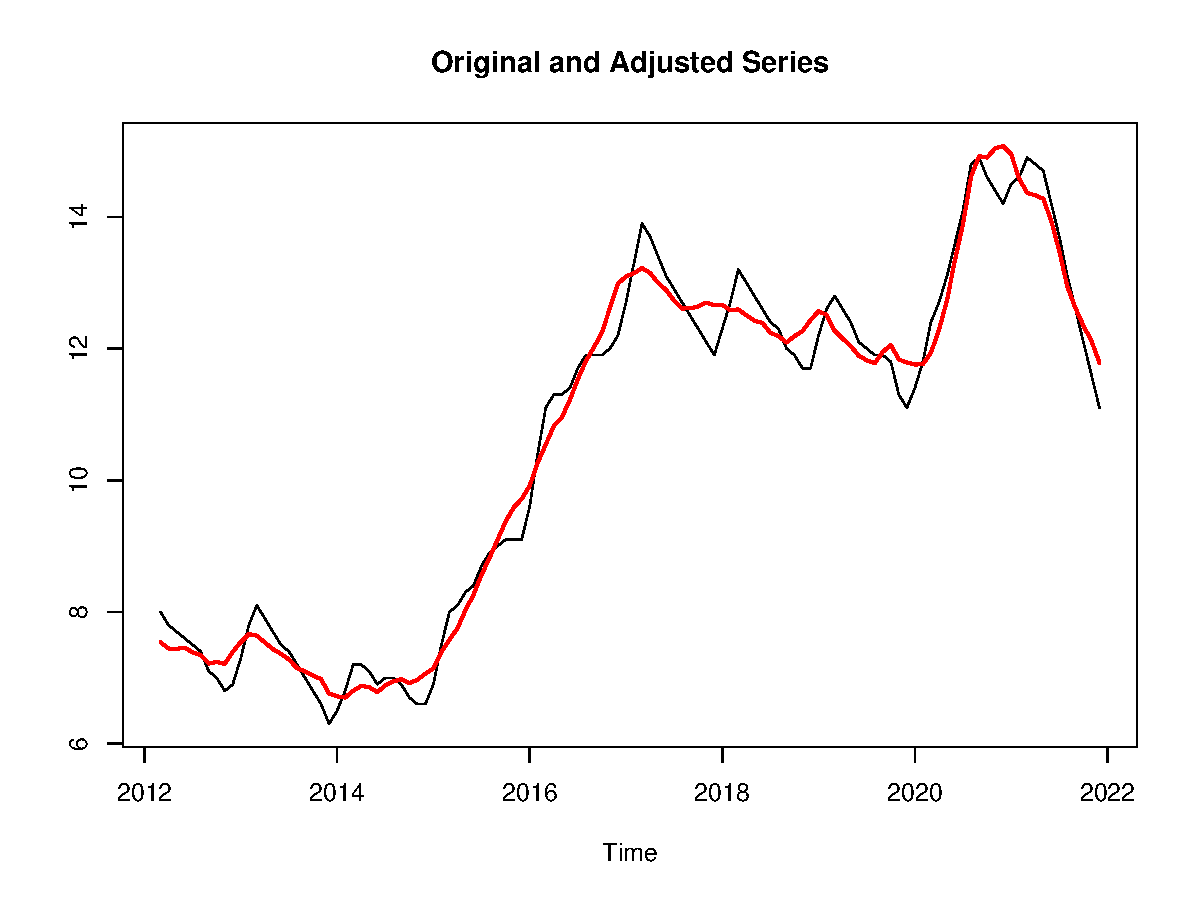
\includegraphics[scale=0.4]{graficos/desemprego_x13.pdf}
	\end{figure}
\end{frame}

\begin{frame}{Separando o ciclo da tendência}
	\begin{halfwideitemize}
		\item Dada uma série de tempo cujo componente sazonal já foi extraído, como separar o componente cíclico da tendência?
		\item Uma abordagem bastante comum consiste em utilizar um {\color{blue}filtro HP}. Formalmente, dada uma série $\{y_t\}_{t=1}^T$,  estimamos a tendência $\{\mu_t\}_{t=1}^T$ resolvendo:
		\begin{equation}
			\min_{\mu_1, \mu_2,\ldots \mu_T} \frac{1}{T} \sum_{t=1}^{T} (y_t - \mu_t)^2 + \frac{\lambda}{T} \sum_{t=2}^{T-1}[(\mu_{t+1}-\mu_t) -(\mu_t - \mu_{t-1})]^2
		\end{equation}
		para uma {\color{blue}penalização} $\lambda > 0$.
		\item $\lambda$ controla o grau de suavidade da tendência estimada (quanto maior $\lambda$, mais suavizado):
		\begin{halfwideenumerate}
			\item Se $\lambda  = 0$, $\hat{\mu}_t = y_t$, i.e. a tendência estimada é a própria série.
			\item Se $\lambda \to \infty$, $\hat{\mu}_t \to \hat{a} + \hat{b} t$, i.e. a tendência torna-se linear (igual à regressão de $y_t$ num intercepto e numa tendência linear).
		\end{halfwideenumerate}
		\item Regra de bolso é usar $\lambda = 1600$ para dados trimestrais, $\lambda =  6,25$ para dados anuais e $\lambda = 129600$ para dados mensais \citep{Ravn2002}.
	\end{halfwideitemize}
\end{frame}



\begin{frame}{Exemplo: taxa de desemprego mensal no Brasil (cont.)}
	\begin{figure}
		\caption{Taxa de desemprego com ajuste via X13 (vermelho) e tendência extraída via filtro HP (azul)}
		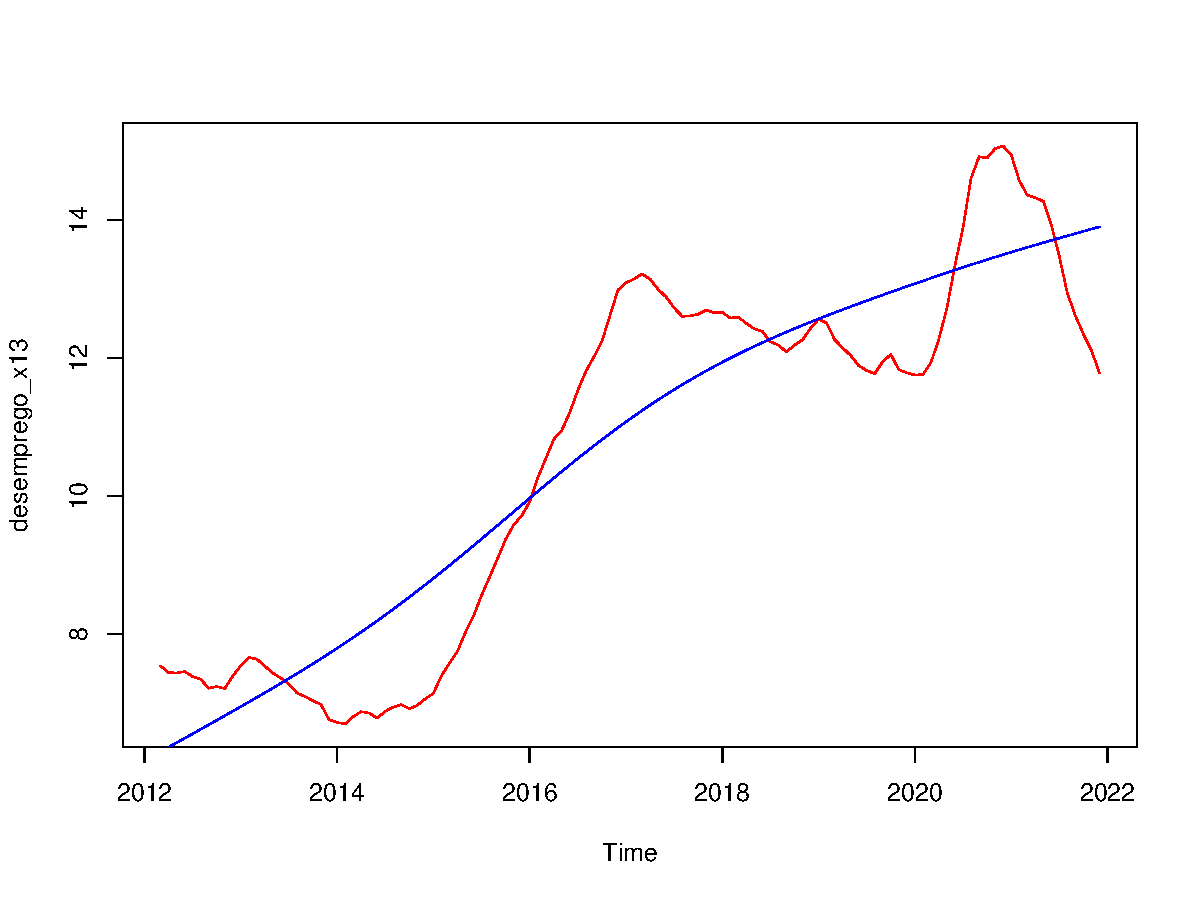
\includegraphics[scale=0.4]{graficos/desemprego_hp.pdf}
	\end{figure}
\end{frame}


\begin{frame}{Filtro HP e instabilidade na ponta}
	\begin{itemize}
		\item Note que, à medida que mais dados são divulgados, os valores da tendência podem mudar.
		\item Esse fenômeno é especialmente acentuado nas observações mais recentes, em que a contribuição de novas observações é especialmente acentuada.
		\begin{itemize}
			\item A esse fenômeno damos o nome de \textbf{instabilidade na ponta}: observações futuras podem fazer nossa estimativa do ciclo mudar radicalmente.
		\end{itemize} 
	\end{itemize}
\end{frame}

\begin{frame}{Instabilidade de ponta: ilustração}
	\begin{figure}
		\caption{Desemprego mensal (ajustado via X13) até janeiro/2024}
		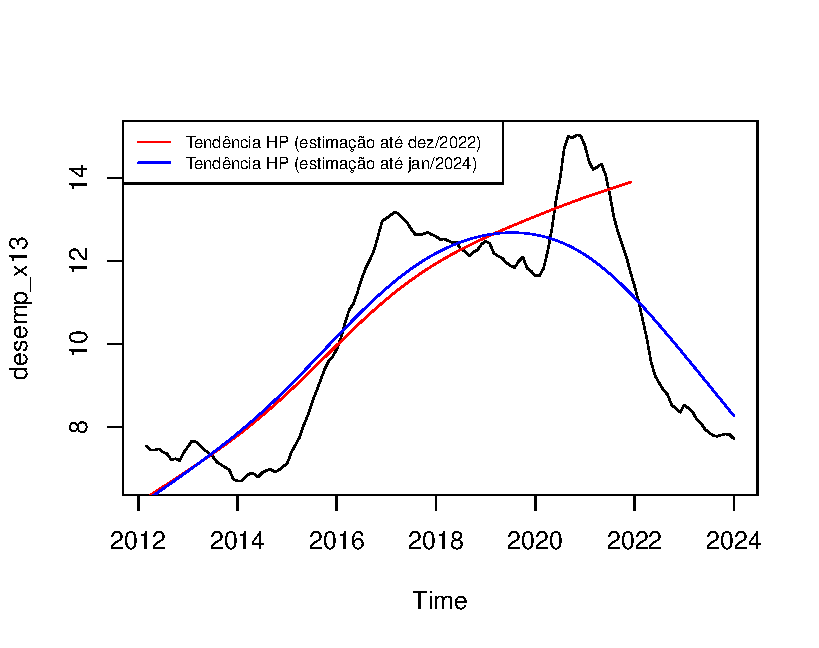
\includegraphics[scale=0.7]{graficos/instabilidade.pdf}
	\end{figure}
\end{frame}

\begin{frame}{Alternativas ao filtro HP: \citet{Hamilton2019}}
	\begin{halfwideitemize}
		\item A instabilidade de ponta, combinada a outras debilidades do filtro HP, leva \citet{Hamilton2019} a sugerir uma outra medida de ciclo.
		\item Sua sugestão é calcular o ciclo como o resíduo $\hat{\nu}_t$ da regressão:
		
		$$y_{t+h} = \alpha+\beta_1 y_{t} + \beta_2 y_{t-1} + \beta_3 y_{t-2} + \beta_4 y_{t-3} + \nu_{t+h} \, ,$$
		onde $h$ é tomado de forma de que a distância entre $t$ e $t+h$ seja de \textbf{dois} anos.
		\begin{itemize}
			\item $h=8$ em dados trimestrais, $h=24$ em dados mensais.
			\item Medida captura o erro que se comete em projetar o que ocorre em $t$, com base no que ocorreu há dois anos.
			\item Ideia é que esse erro capturaria fatores cíclicos.
		\end{itemize}
	\end{halfwideitemize}
\end{frame}

\begin{frame}{Aplicação de \citet{Hamilton2019} aos dados de desemprego}
	\centering
	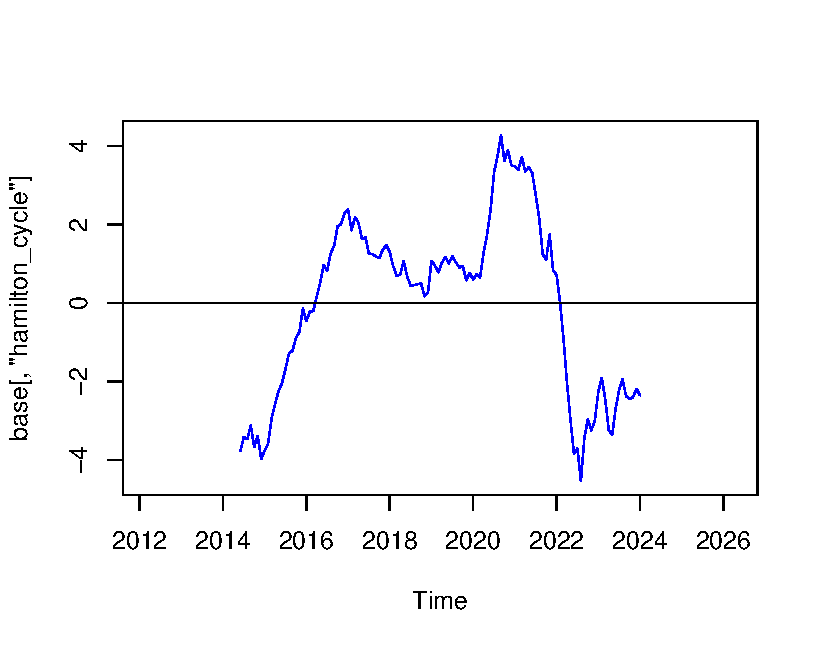
\includegraphics[scale=0.7]{graficos/hamilton.pdf}
\end{frame}

\begin{frame}{Decomposição de Beveridge-Nelson}
	\begin{itemize}
		\item A decomposição de Hamilton é bastante similar a um procedimento, sugerido por \citet{Beveridge1981}, para se separar a tendência estocástica da parte estacionária de um processo I(1).
		\item Decomposição de Beveridge-Nelson toma a parte estacionária de um processo I(1) como:
		
		$$\nu^{\text{BN}}_t = y_t - \lim_{s \to \infty} \mathbb{E}[y_{t+s}|y_t,y_{t-1},\ldots]$$
		i.e. a diferença entre $y_t$ e uma projeção de longo prazo, feita com base em toda o histórico de $y$ até $t$.
		\item Se processo também apresenta tendência determinística $a_0 t$ em nível, fazemos: 
			$$\nu^{\text{BN}}_t = y_t - \lim_{s \to \infty} ( \mathbb{E}[y_{t+s}|y_t,y_{t-1},\ldots] - a_0 s)$$
			\item Decomposição pode ser estimada ajustando um modelo preditivo para $\Delta y_t$, e computando projeções fora da amostra para um horizonte longo, observando que $y_{t+s} = y_t + \Delta y_{t+1} + \ldots \Delta y_{t+s}$.
	\end{itemize}
\end{frame}
\appendix
	\begin{frame}[allowframebreaks]{Bibliografia}
	\printbibliography
	\end{frame}
\end{document}